%----------------------------------------------------------------------------------------
%	LATEX SAMENVATTING TEMPLATE
%	Versie 1.3 (9 september 2014)
%	Opmerkingen of feedback naar Robert van Wijk
%					(robertvanwijk@uva.nl)
%----------------------------------------------------------------------------------------

%----------------------------------------------------------------------------------------
%	PACKAGES EN DOCUMENT CONFIGURATIE
%----------------------------------------------------------------------------------------

\documentclass[a4paper,12pt]{article}
\usepackage{algorithm2e}
\usepackage[dutch]{babel}
\usepackage{fancyhdr}
\usepackage{graphicx}
\usepackage{hyperref}
\usepackage{lastpage}
\usepackage{longtable}
\usepackage{lipsum}
\usepackage{tabu}
\usepackage{tikz}
	\usetikzlibrary{mindmap,backgrounds}
\usepackage{verbatim}

%----------------------------------------------------------------------------------------
%	DOCUMENT INFORMATIE
%----------------------------------------------------------------------------------------
%Geef bij ieder command het juiste argument voor deze opdracht. Vul het hier in en het komt op meerdere plekken in het document correct te staan.

\newcommand{\opdracht}{Samenvatting}			%Voor deze opdracht niet veranderen
\newcommand{\titel}{Vermingvuldigen in computer architectuur}	%Nummer en titel van het samengevatte hoofdstuk
\newcommand{\studentA}{Steven Raaijmakers}			%Vul je eigen voor- en achternaam in
\newcommand{\uvanetidA}{10804242}
\newcommand{\tutor}{Ellen van Leeuwen}				%Vul de voor- en achternaam van je tutor in
\newcommand{\PAVgroep}{COBOL (C1)}		%ALGOL (A1), Amiga E (A2), etcetera
\newcommand{\datum}{\today}					%Pas aan als je niet de datum van vanaag wilt hebben

%----------------------------------------------------------------------------------------
%	AUTOMATISCHE HEADER & FOOTER
%----------------------------------------------------------------------------------------
%Hoef je niets aan te veranderen

\pagestyle{fancy}
  \lhead{
\includegraphics[width=7cm]{logoUvA}}		%Zorg dat het logo in dezelfde map staat
  \rhead{\footnotesize \textsc {Samenvatting\\ \titel}}
  \lfoot
    {
	\footnotesize \studentA (\uvanetidA)
    }
  \cfoot{}
  \rfoot{\small \textsc {Pagina \thepage\ van \pageref{LastPage}}}
  \renewcommand{\footrulewidth}{0.5pt}

\fancypagestyle{firststyle}
 {
  \fancyhf{}
   \renewcommand{\headrulewidth}{0pt}
   \chead{
\includegraphics[width=7cm]{logoUvA}}
   \rfoot{\small \textsc {Pagina \thepage\ van \pageref{LastPage}}}
 }

\setlength{\topmargin}{-0.3in}
\setlength{\textheight}{630pt}
\setlength{\headsep}{40pt}

%----------------------------------------------------------------------------------------
%	AUTOMATISCHE TITEL
%----------------------------------------------------------------------------------------
%Hoef je niets aan te veranderen

\begin{document}
\thispagestyle{firststyle}
\begin{center}
	\textsc{\Large \opdracht}\\[0.2cm]
		\rule{\linewidth}{0.5pt} \\[0.4cm]
			{ \huge \bfseries \titel}
		\rule{\linewidth}{0.5pt} \\[0.2cm]
	{\large \datum  \\[0.4cm]}

	\begin{minipage}{0.4\textwidth}
		\begin{flushleft}
			\emph{Student:}\\
			{\studentA \\ {\small \uvanetidA \\[0.2cm]}}
		\end{flushleft}
	\end{minipage}
~
	\begin{minipage}{0.4\textwidth}
		\begin{flushright}
			\emph{Tutor:} \\
			\tutor \\[0.2cm]
			\emph{PAV-groep:} \\
			\PAVgroep \\[0.2cm]
		\end{flushright}
	\end{minipage}\\[1 cm]
\end{center}

%----------------------------------------------------------------------------------------
%	ALINEA-METHODE
%----------------------------------------------------------------------------------------
%Zet hieronder je tekst. Denk aan de indeling in alinea's en eventueel section headers!

\section{Verhogen multiplicand en multiplier}

Wanneer de waardes van de multiplicand en de multiplier verhoogd worden, geeft het product een foutief resultaat weer. Zo geeft de 0x een 
hexadecimaal getal weer, en de 0b binaire getallen. 

\section{CPI meten}
Het CPI van een multiply instruction kan gemeten worden doordat op de 423ste tijdseenheid de ready naar 1 verspringt. Omdat de clock cycle uit 10 verschillende 
eenheden bestaat, zou dit betekenen dat er dus 42,3 clock cycles zijn. Dit wordt vervolgens gedeeld door 12 wat een uiteindelijk CPI geeft van 3,52. 

\section{Toevoegen hardware multiplier}
Als de SingleCycle architecture een hardware multiplier een toegoegd krijgt zal het totale aantal control lines en data lines toenemen.

\subsection{Effect op cycles}
Wanneer er een hardware multiplier wordt toegevoegd zullen tevens de cycles  langer worden, maar bij een multiplier instructie zal dit uiteindelijkgeen vertraging opleveren. 
Wanneer hetzelfde wordt gedaan met bijvoorbeeld add-instructies zullen sommige cycles onnodig lang worden waardoor dit uiteindelijk wel vertraging oplevert. 

\section{MULT instructie}
De Opcode van een MULT instruction: 011000. Vervolgens wordt er via de truth-tabel gecontroleerd of deze instructie 
inderdaad voorkomt. Wanneer deze instructie gevonden wordt; wordt deze uitgevoerd. 

\section{Oplossen hazards}
Het oplossen van een fout die ontstaat wanneer de ALU en de multiplier hetzelfde dapath voor de register file gebruiken kan door een extra multiplexer aan te sluiten. Hiermee kun je controleren welk 
signaal er moet worden doorgegeven. 

%----------------------------------------------------------------------------------------
%	MINDMAP
%----------------------------------------------------------------------------------------
%Voorbeeld voor gebruik tijdens de latere weken, verwijder de \begin en \end{comment} om te zien.

\begin{comment}
\begin{figure}
\centering
\begin{tikzpicture}[mindmap, grow cyclic, text width=2.7cm, every node/.style=concept, concept color=orange!40,
    level 1/.append style={level distance=4.0cm,sibling angle=72},
    level 2/.append style={level distance=2.5cm,sibling angle=60},]

\node{Academische Vaardigheden}
    child [concept color=blue!30] { node {Academische houding}
	child { node {Fraude en plagiaat } }
	child { node {Feedbacke en reflectie } }
	child { node {Mondeling communicatie } }
	child { node (saa) {Studeren als academicus } }
    }
    child [concept color=yellow!30] { node (onv) {Onderzoeks-vaardigheden}
	child { node { Literatuur-onderzoek } }
	child { node { Technisch rapport } }
     }
    child [concept color=green!40] { node {Schrijfvaar-digheden}
	child { node { Schrijf-proces } }
	child { node { Weten-schappelijke schrijfstijl } }
	child { node { Taal-gebruik } }
	child { node { Figuren en tabellen } }
    }
    child [concept color=teal!40]{ node {Presentatie-vaardigheden}
	child { node { Presen-taties } }
	child { node { Poster-presen-taties } }
    }
    child [concept color=purple!50]{ node {Projectvaar-digheden}
	child { node { Teamrollen } }
	child { node { Valkuilen bij samenwerken } }
    };

\begin{pgfonlayer}{background}
    \draw [circle connection bar]
      (saa) edge (onv);
\end{pgfonlayer}

\end{tikzpicture}

\caption{Mindmap van de Academische Vaardigheden.}
\end{figure}
\end{comment}

%----------------------------------------------------------------------------------------
%	KOLOMMENSCHEMA
%----------------------------------------------------------------------------------------
%Voor gebruik tijdens de latere weken, verwijder de \begin en \end{comment}.

\begin{comment}
\begin{longtabu} to \linewidth {l|l|X|X}
\caption{Leeg kolomschema} \\
\rowfont\bfseries Hoofdzaak & Aspect & Inhoud & Voorbeeld \\ \hline
\endhead

\multicolumn{4}{r}{{Vervolgd op de volgende pagina}} \\
\endfoot

\endlastfoot

Hoofdzaak1
& Aspect1
& Inhoud1


Hoofdzaak2
& Aspect1
& Inhoud1
& Voorbeeld1
\\ \cline{2-4}

& Aspect2
& Inhoud2
& Voorbeeld2
\\ \hline

Hoofdzaak3
& Aspect1
& Inhoud1
& Voorbeeld1
\\ \cline{2-4}

& Aspect2
& Inhoud2
& Voorbeeld2
\\ \hline

\end{longtabu}
\end{comment}

%----------------------------------------------------------------------------------------
%	HET EINDE
%----------------------------------------------------------------------------------------
\end{document}
